\scanpage{14}
\mspage{13}

3) Être homéom. à $S^n$. On trouve p.ex. sur $S^{n+1}$ munie de deux pts \inserted{distincts} (antipodiques, si on veut) $a,b$, une théorie des \unsure{2} décompositions par des $S^n$.

\figure{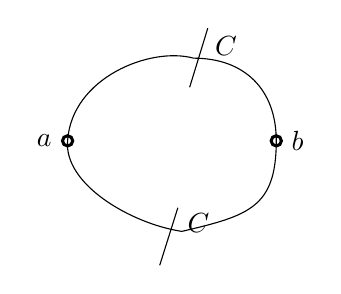
\begin{tikzpicture}[x=1cm,y=1cm]
\draw (0,0) .. controls (.05,.8) and (1.05,1.2) .. (1.6,1.05) .. controls (2.25,1.05) and (2.65,.65) .. (2.65,0) .. controls (2.65,-.85) and (2.3,-.95) .. (1.45,-1.15) .. controls (.8,-1.05) and (-.05,-.55) .. (0,0);
\draw[line width=1.1pt] (0,0) circle (.065) (2.65,0) circle (.065);
\draw (1.55,.68)--(1.78,1.43) (1.17,-1.58)--(1.4,-.85);
\node[left] at (-.08,0){$a$};\node[right] at (2.72,0){$b$};
\node[right] at (1.75,1.2){$C$};\node[right] at (1.4,-1.05){$C$};
\end{tikzpicture}}

On peut aussi exiger, sur un lieu distinct des extrémités, que la structure de $X$ au voisinage de $C$ soit celle de $C\times]-1,1[$, avec $C$ correspondant à $C_0=C\times\{0\}$, et les deux ``rives'' $C\times]-1,0[$, $C\times]0,1[$ étant contenues resp. dans les deux ficelles composantes $X_{A,C}$, $X_{\unsure{B},C}$.

\rotatebox{90}{\reflectbox{\unsure{EXTRA STRONG}}}
\rotatebox{90}{\reflectbox{\unsure{EXTRA STRONG}}}
\mspage{13}
